\chapter{关系模型}

\begin{introduction}[期末考试提纲]
    \item 笛卡尔积
    \item 关系模型三要素
    \item 关系模型的完整性
    \item 全关系系统的十二条准则
    \item 关系运算
    \item 元组演算表达式
    \item 域关系演算表达式
    \item 用关系代数表达关系数据操作
\end{introduction}

\section{关系基本概念}

\begin{definition}[域(Domain)]
具有相同数据类型的一组值的集合.
如整数集合、字符串集合、全体学生集合.
\end{definition}

\begin{definition}[笛卡尔积(Cartesian Product)]
一组域$D_1,D_2,...,D_n$的\textcolor{red}{笛卡尔积}为:
\begin{align*}
    D_1\times D_2\times \cdots\times D_n = \{(d_1,d_2,...,d_n)|d_i\in D_i, i=1,2,...,n\}.
\end{align*}
笛卡尔积的元素$(d_1,d_2,...,d_n)$称作$n$元组(tuple).

元组的每一个值$d_i$被称作分量(component).

若$D_i$的基数为$m_i$, 则笛卡尔积的基数为$\prod_{i=1}^{n}m_i$.
\end{definition}

\begin{definition}[关系]
笛卡尔积$D_1\times D_2\times \cdots\times D_n$的子集称作在域$D_1,D_2,...,D_n$上的\textcolor{red}{关系}. 用$R(D_1,D_2,...,D_n)$表示. $R$是关系的名字, $n$是关系的度或目.

关系是笛卡尔积中\textcolor{red}{有意义}的子集.
\end{definition}

关系的性质:
\begin{enumerate}
    \item $P_1$: 列是同质的, 是同一类型的数据, 即每一列中的分量来自同一域.
    \item $P_2$: 不同的列可以来自同一域, 每列必须有不同的属性名. (一元联系、类型相同的属性)
    \item $P_3$: 行列的顺序无关紧要.
    \item $P_4$: 任意两个元组不能完全相同 (集合内不能有相同的两个元素)
    \item $P_5$: 每一分量必须是不可再分的数据, 称其为作满足第一范式(1NF)的关系. 
\end{enumerate}

\section{关系模型三要素}

关系模型的三要素:
\begin{enumerate}
    \item 数据结构.
    \item 数据操作.
    \item 数据完整性.
\end{enumerate}

\subsection{数据结构}

关系模型的数据结构就是\textcolor{red}{关系}: 实体集和联系都表示为关系.

\begin{definition}[候选码(Candidate Key)]
关系中的一个属性组, 其值能唯一标识一个元组. 
若从属性组去掉任何一个属性, 它就不具有这一性质了, 这样的属性组称为候选码.
\end{definition}

\begin{definition}[主属性]
任何一个候选码中的属性被称为主属性.
\end{definition}

\begin{definition}[主码(Priamry Key, PK)]
进行数据库设计时, 从一个关系的多个候选码中选定一个作为主码.
\end{definition}

\begin{definition}[外码(Foreign Key, FK)]
关系$R$中的一个属性组, 它不是$R$的码, 但它与另一个关系$S$的码相
对应, 称这个属性组为$R$的外码.
\end{definition}

\begin{definition}[关系模式]
关系的描述, 记为$R(A_1,A_2,...,A_n)$, 包括:
\begin{enumerate}
    \item 关系名、关系中的属性名.
    \item 属性向域的映像, 通常说明为属性的类型、长度等.
    \item 属性间的数据依赖关系, 比如在特定的时间和教室只能安排一门课.
\end{enumerate}
关系模式是稳定的.
\end{definition}

\begin{definition}[关系]
关系是某一时刻对应某个关系模式的内容(元组的集合). 关系是某一时刻的值, 是随时间不断变化的.
\end{definition}

\begin{definition}[关系型数据库]
\begin{enumerate}
    \item 型: 关系模式的集合, 数据库描述. 数据库的内涵(Intension).
    \item 值: 是某一时刻关系的集合. 数据库的外延(Extension).
\end{enumerate}
\end{definition}

\subsection{数据操作}

关系操作是集合操作. 操作的对象及结果都是集合. 是一次一集合 (Set-at-a-time)的方式.

非关系型的数据操作方式是一次一记录(Record-at-a-time).

关系数据语言的特点:
\begin{enumerate}
    \item 一体化: 对象单一, 都是关系, 因此操作符也单一
    \item 非过程化: 用户只需提出“做什么” , 无须说明“怎么做”. 存取路径的选择和操作过程由系统自动完成
    \item 面向集合的存取方式: 一次一关系.
\end{enumerate}

抽象的关系模型查询语言:
\begin{enumerate}
    \item 关系代数. 过程查询语言.
    \item 关系演算: 元组关系演算、域关系演算. 非过程查询语言.
\end{enumerate}

SQL(介于关系代数和关系验算之间, by IBM)、QUEL(基于 Codd 提出元组关系演算语言ALPHA)、QBE.

\subsection{数据完整性}

\begin{definition}[关系模型完整性]
关系模型完整性由三部分组成:
\begin{enumerate}
    \item 实体完整性
    \item 参照完整性
    \item 用户定义完整性
\end{enumerate}
\end{definition}

\begin{definition}[实体完整性]
关系的主码中的属性值不能为空值. (保证其实体存在.)
\end{definition}

\begin{definition}[参照完整性]
如果关系$R_2$的外码$F_k$与关系$R_1$的主码$P_k$相对应, 
则$R_2$中每个元组的$F_k$值或者等于$R_1$中某个元组的$P_k$值, 或者为空值.

如果关系$R_2$的某个元组$t_2$参照了关系$R_1$的某个元组$t_1$, 则$t_1$必须存在, 
也即必须与客观存在的实体发生联系.
\end{definition}

\begin{figure}[H]
    \centering
    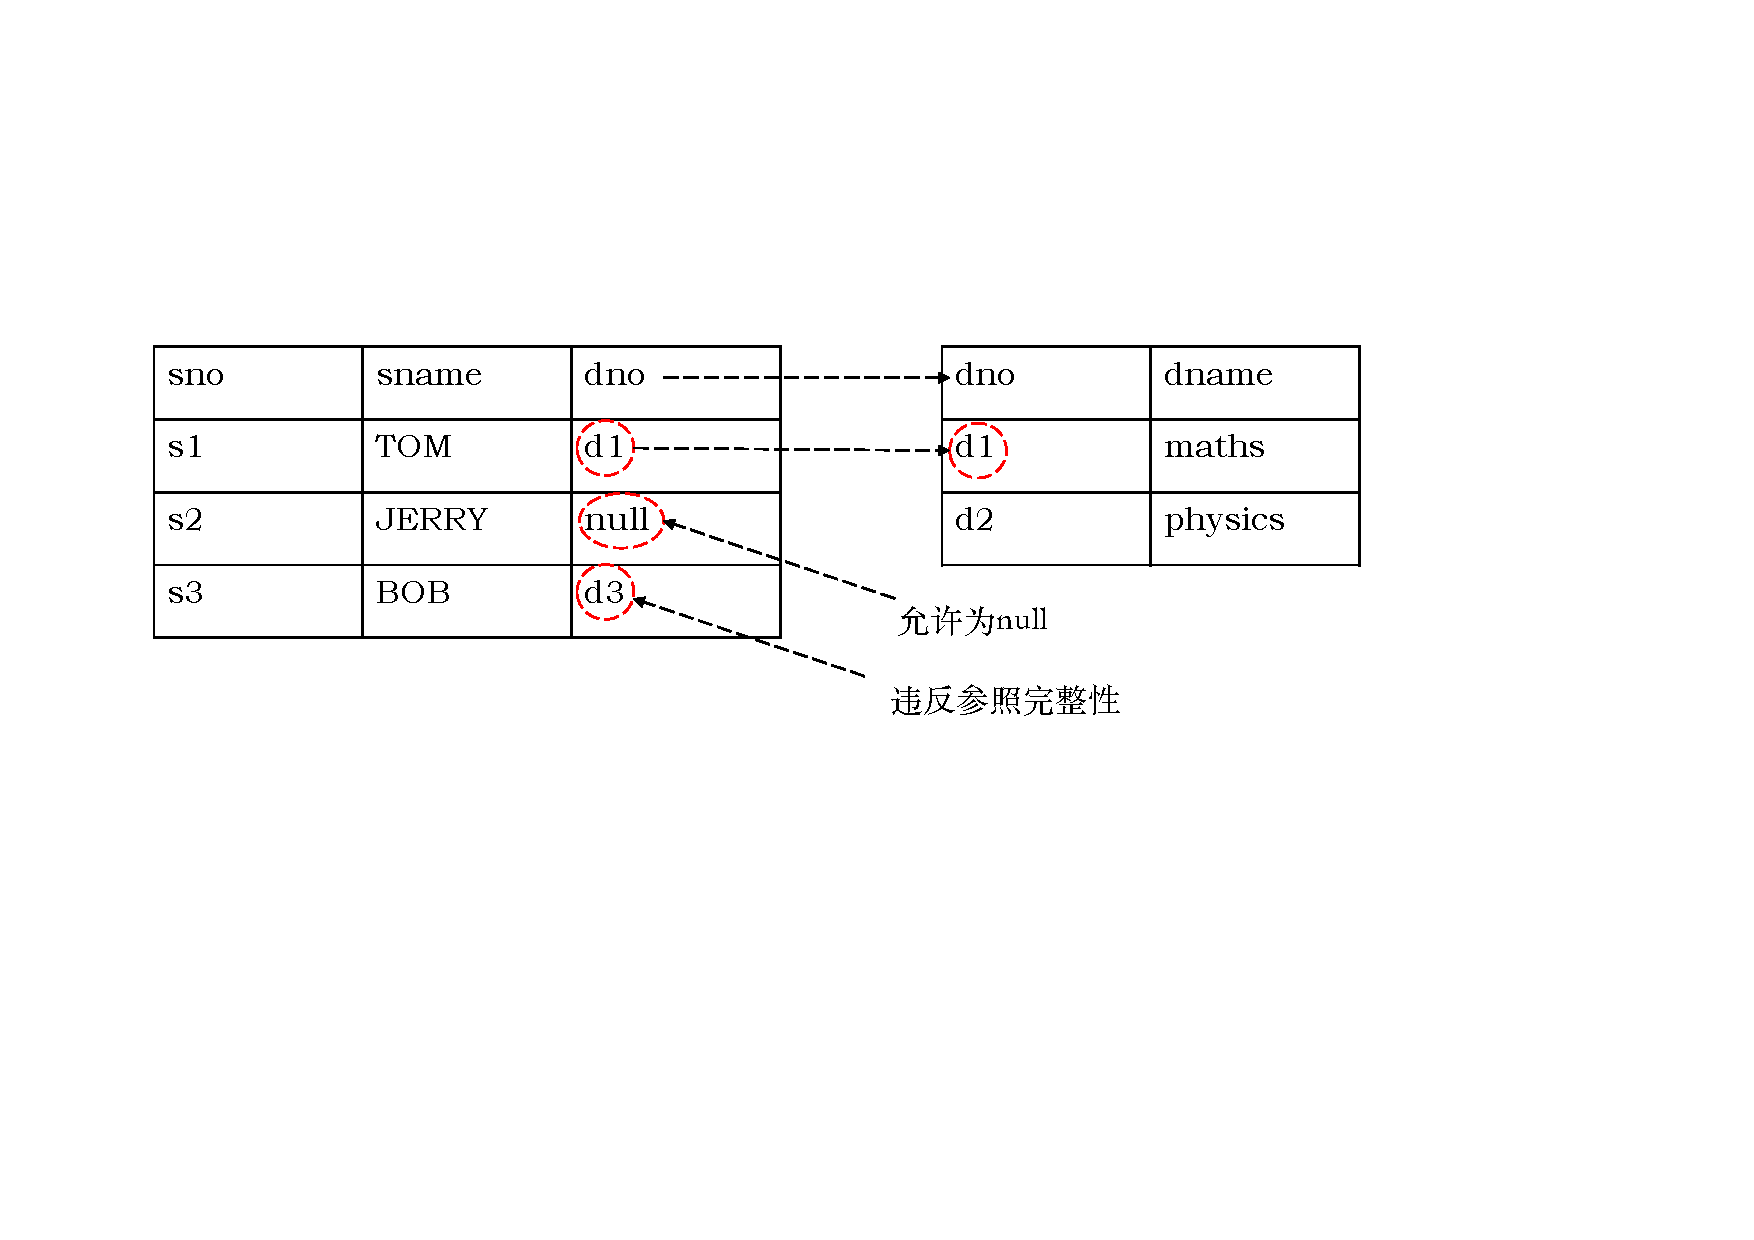
\includegraphics[width=.6\textwidth]{./figure/参照完整性.pdf}
    \caption{参照完整性}
\end{figure}

\begin{definition}[用户完整性]
用户针对具体应用环境定义的完整性约束条件.
\end{definition}

实体完整性和参照完整性由系统自动支持, 系统提供定义和检验用户定义的完整性的机制.

\section{关系代数运算}

\begin{figure}[H]
    \centering
    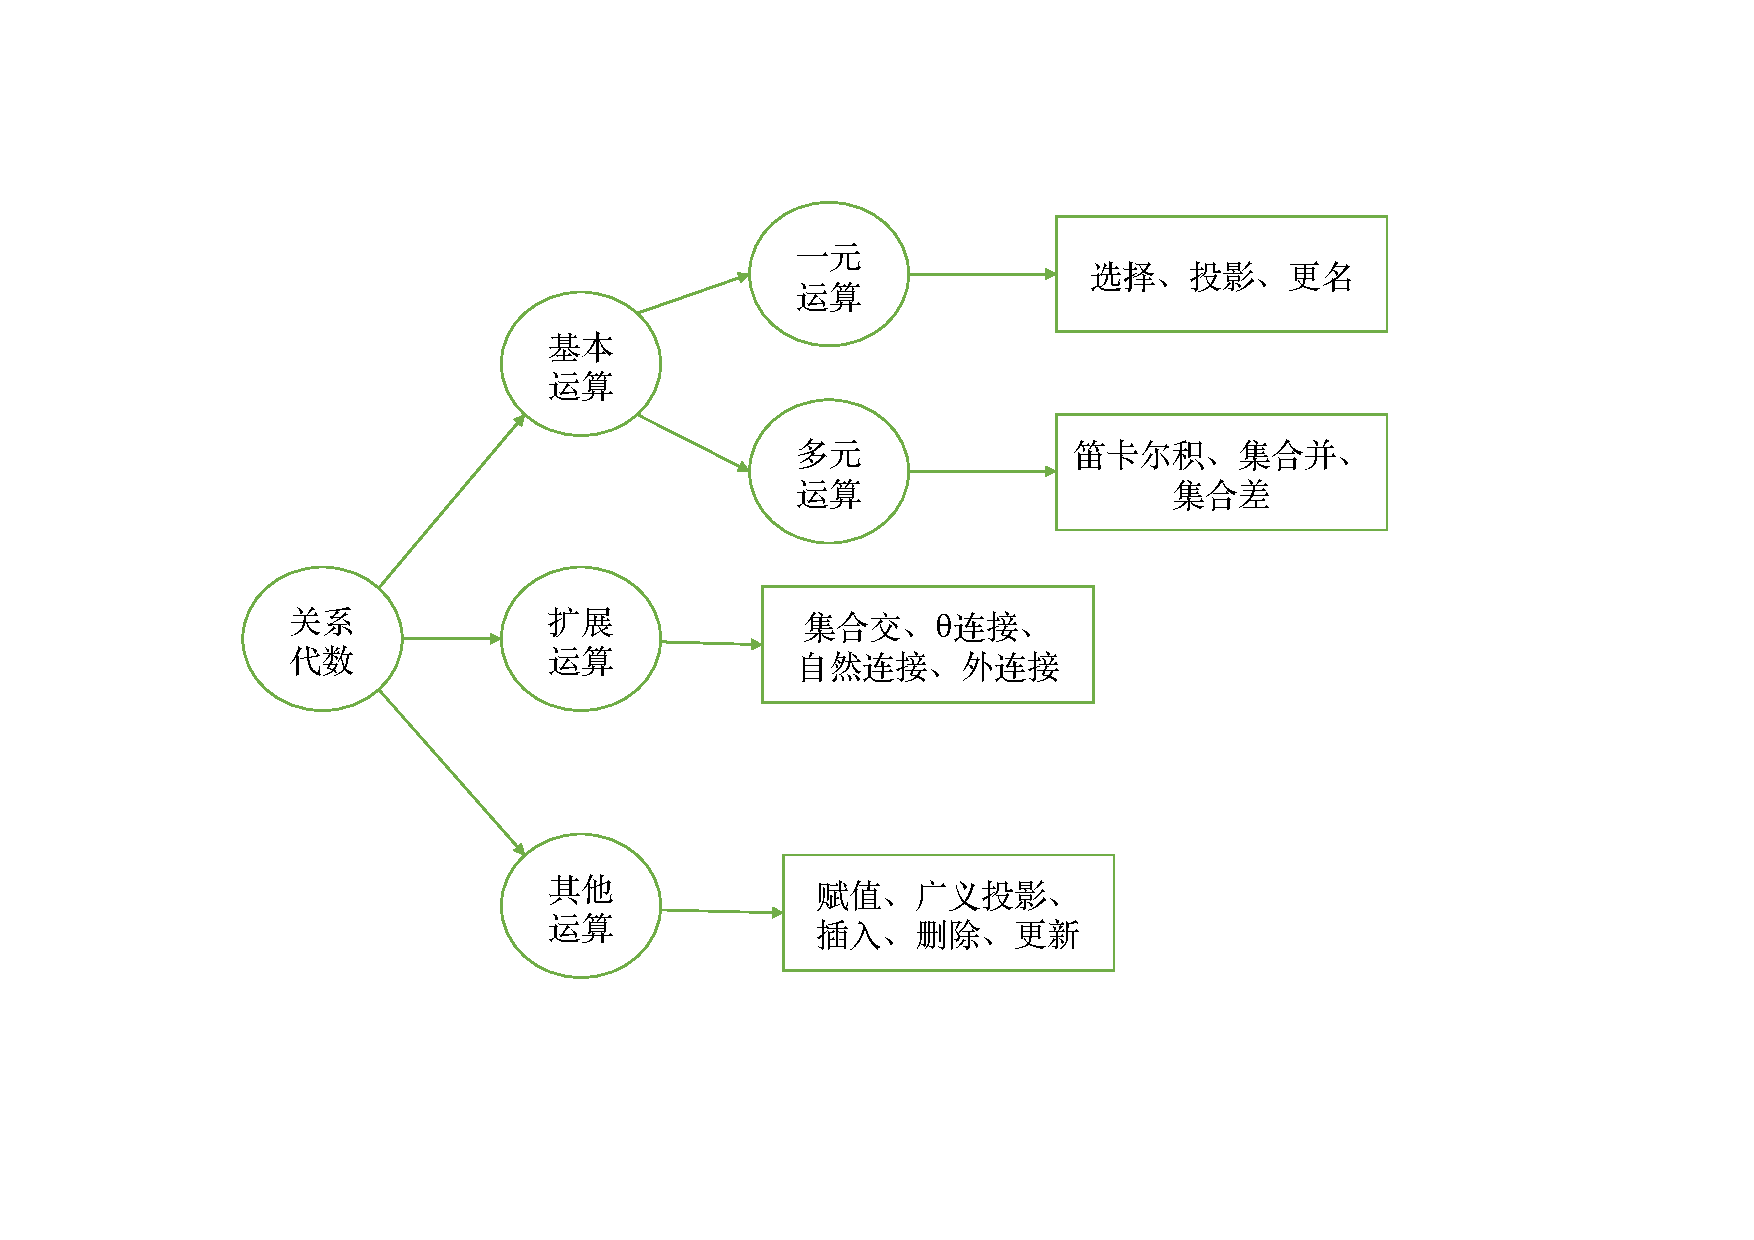
\includegraphics[width=.6\textwidth]{./figure/关系代数.pdf}
\end{figure}

\subsection{基本关系代数运算}

\subsubsection{一元运算}

\begin{definition}[选择运算]
在关系中选择给定条件的元组(行角度):
\begin{align*}
    \sigma_F(R)=\{t|t\in R,F(t)=\text{true}\}.
\end{align*}
$F$由逻辑运算符连接算术表达式而成.
\end{definition}

\begin{definition}[投影运算]
从关系中取若干列组成新的关系(从列的角度):
\begin{align*}
    \Pi_A(R) = \{t[A]|t\in R\}, A \subseteq R.
\end{align*}
\end{definition}

投影的结果要去掉相同的行:
\begin{figure}[H]
    \centering
    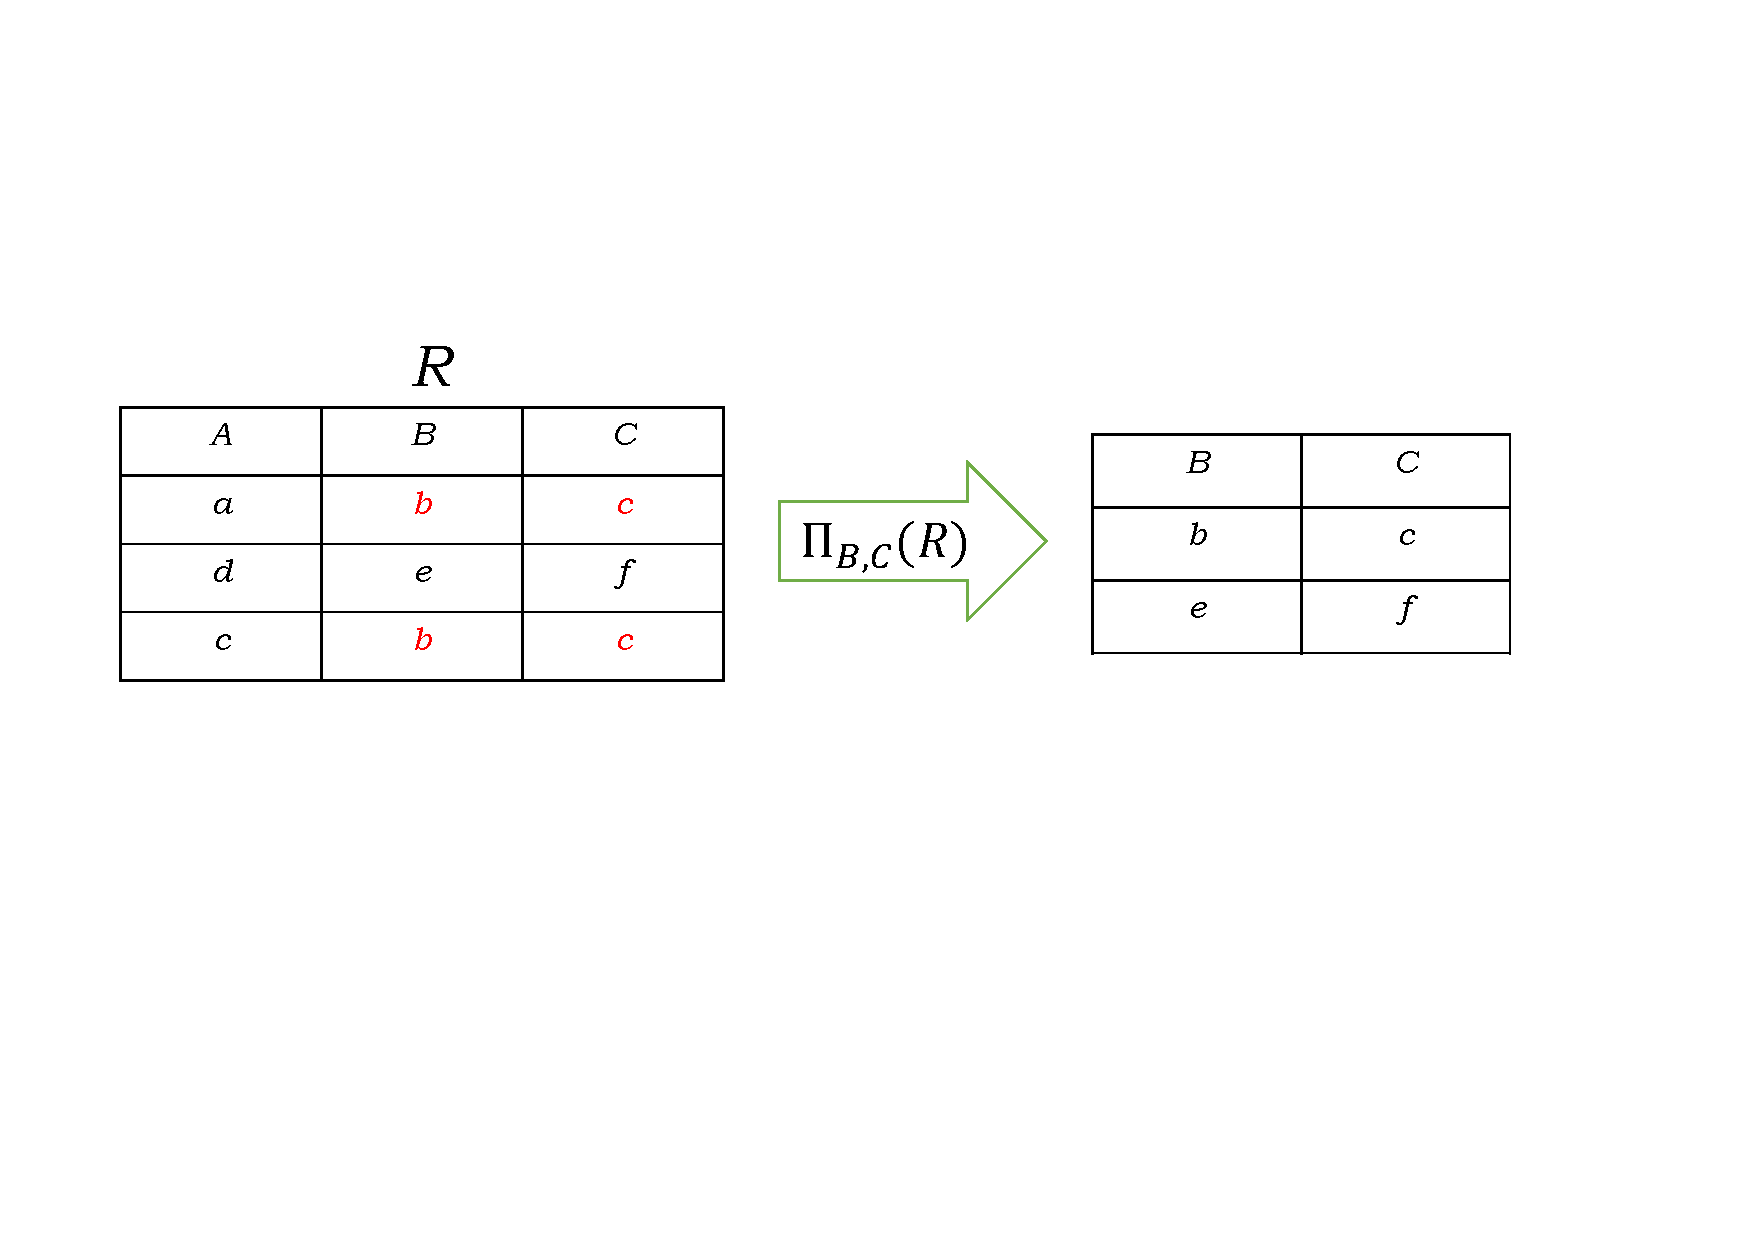
\includegraphics[width=.7\textwidth]{./figure/投影.pdf}
    \caption{投影运算要去掉相同的行}
\end{figure}

\begin{definition}[更名运算]
将关系$R$更名为$S: \rho_S(R)$; 将计算表达式$E$更名为关系$S: \rho_{S(A_1,A_2,...,A_n)}(E)$.
\begin{enumerate}
    \item 将更名运算施加到关系上, 得到具有不同名字的同一关系
    \item 当同一关系多次参与同一运算时需要更名
\end{enumerate}
\end{definition}

\subsubsection{多元运算}

\begin{definition}[并运算]
\begin{align*}
    R\cup S =\{r|r\in R\lor r \in S\}.
\end{align*}
关系$R$和$S$进行并运算的前提是它们必须是相容的.
\begin{enumerate}
    \item 关系$R$和$S$必须是同元的, 其属性数目必须相同.
    \item 对$\forall i$, $R$的第$i$个属性和$S$的第$i$个属性的域必须相同.
\end{enumerate}
\end{definition}

\begin{example}
选修了001号或002号课程的学生号.
\begin{align*}
    &\Pi_{\text{sno}}(\sigma_{\text{cno}=001\lor \text{cno}=002}(\text{SC})) \\
    &\Pi_{\text{sno}}(\sigma_{\text{cno}=001}(\text{SC})\lor \sigma_{\text{cno}=002}(\text{SC}))
\end{align*}
\end{example}

\begin{definition}[差运算]
\begin{align*}
    R-S =\{r|r\in R\land r \not\in S\}.
\end{align*}
\end{definition}

\begin{example}
求选修了001号但未选修002号课程的学生号.
\begin{align*}
    &\Pi_{\text{sno}}(\sigma_{\text{cno}=001}(\text{SC})) - \Pi_{\text{sno}}(\sigma_{\text{cno}=002}(\text{SC})) \\
   &\Pi_{\text{sno}}(\sigma_{\text{cno}=001\lor \text{cno}\neq 002}(\text{SC}))
\end{align*}
\end{example}

\begin{definition}[连串(Concatenation)]
$r=(r_1,r_2,...,r_n)$, $s=(s_1,s_2,...,s_m)$, $r$与$s$的连串定义为:
\begin{align*}
    \widehat{rs} = (r_1,r_2,...,r_n,s_1,s_2,...,s_m).
\end{align*}
\end{definition}

\begin{definition}[笛卡尔积]
\begin{align*}
    R\times S=\{\widehat{rs}|r\in R\land s\in S\}.
\end{align*}
\begin{itemize}
    \item $R\times S$的度为$R$和$S$的度之和.
    \item $R\times S$的元组个数为$R$和$S$的元组个数之积.
\end{itemize}
\end{definition}

\begin{example}
求选修c1课程的学生姓名.
\end{example}

\begin{figure}[H]
    \centering
    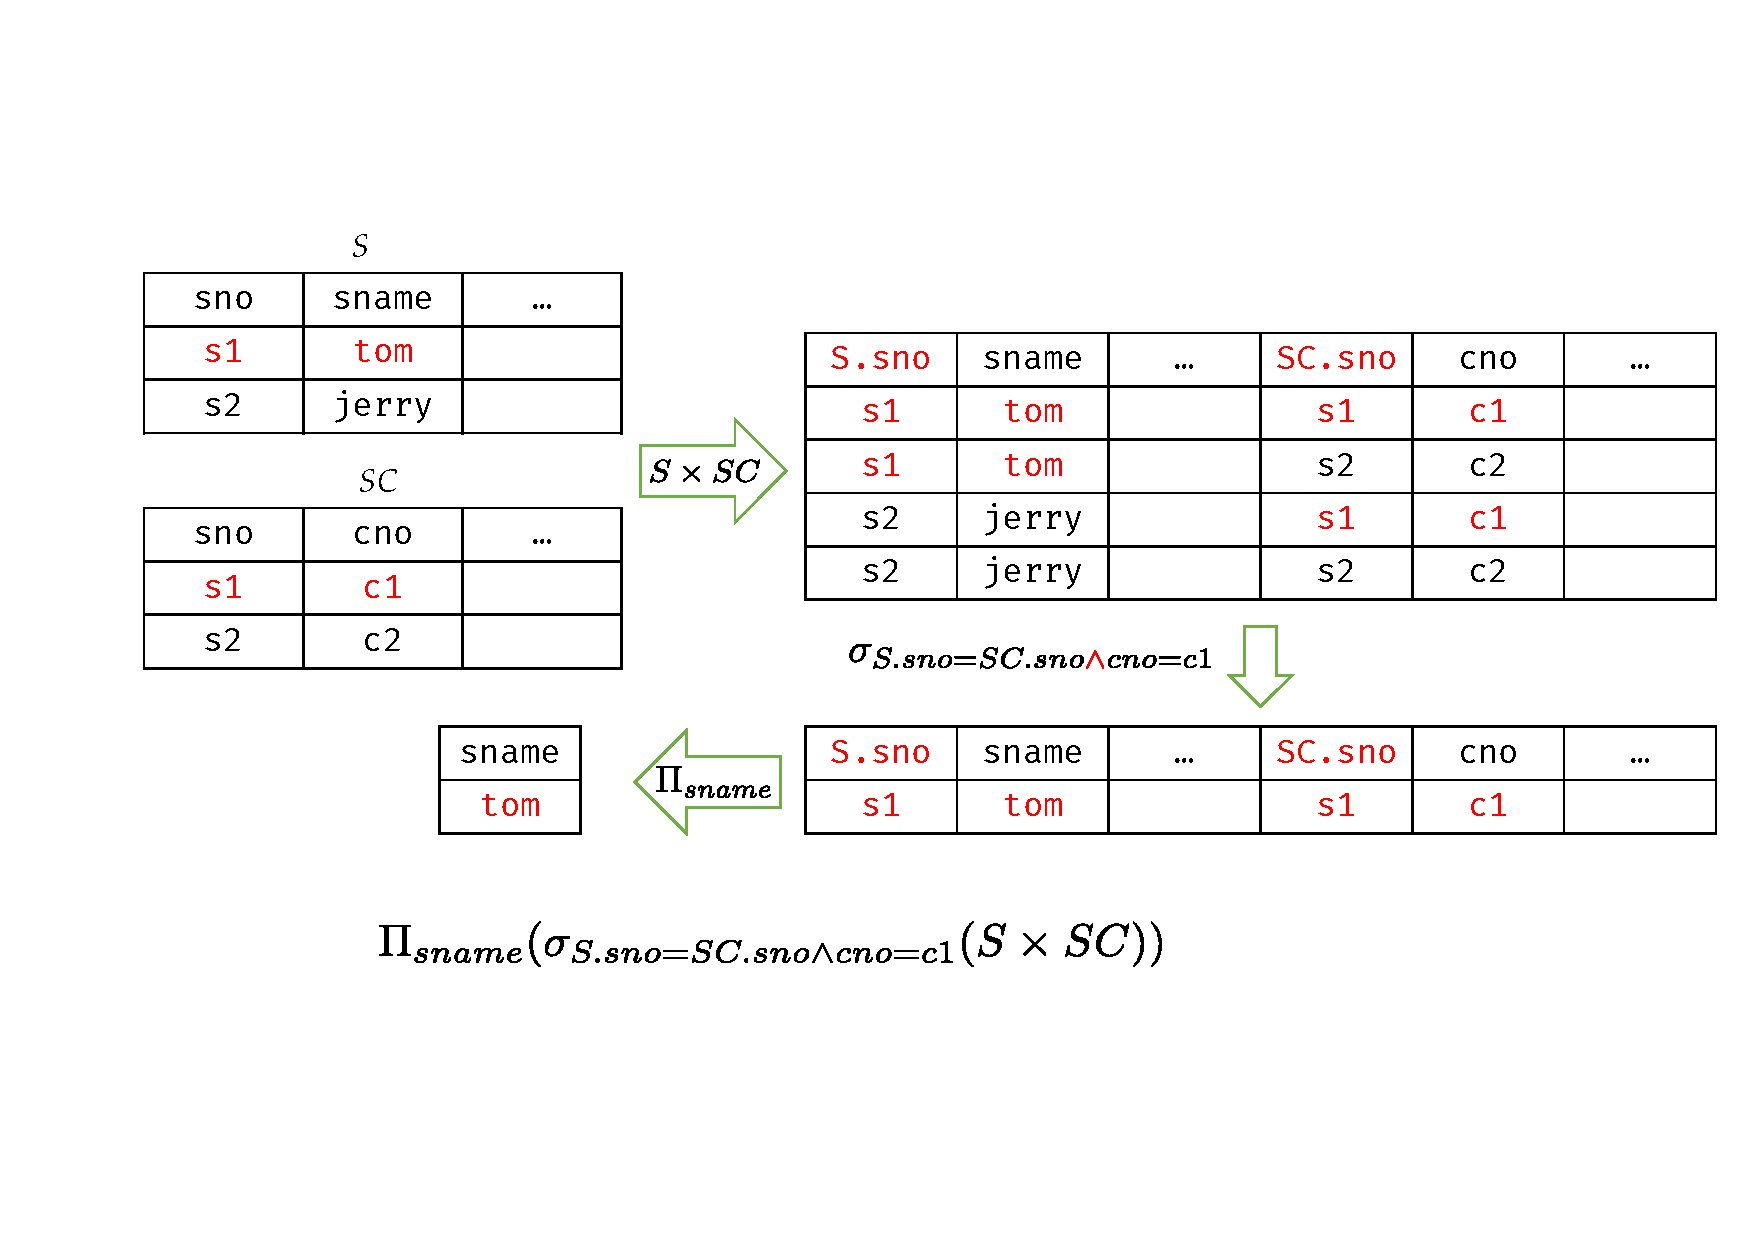
\includegraphics[width=.75\textwidth]{./figure/笛卡尔积的使用.pdf}
    \caption{笛卡尔积的使用}
\end{figure}

\begin{example}
求数学成绩比王红同学高的学生姓名.
\end{example}
\begin{align*}
    \Pi_{S.\text{姓名}}\left(\sigma_{R.\text{姓名}=\text{王红}\land R.\text{课程}=\text{数学}\land S.\text{课程}=\text{数学} \land R.\text{成绩} < S.\text{成绩}} (R\times \rho_S(R))\right)
\end{align*}

\subsection{扩展关系代数运算}

\begin{definition}[交运算]
\begin{align*}
    R\cap S =\{r|r\in R\land r \in S\}.
\end{align*}
$R\cap S = R-(R-S)$.
\end{definition}

\begin{example}
求同时选修了001号和002号课程的学生号.
\end{example}
\begin{align*}
    &\Pi_{\text{sno}}(\sigma_{\text{cno}=001}(\text{SC})) \cap \Pi_{\text{sno}}(\sigma_{\text{cno}=002}(\text{SC})) \\
    &\Pi_{\text{sno}}(\sigma_{\text{cno}=001\land \text{cno}=002}(\text{SC}))
\end{align*}

\begin{definition}[$\theta$连接]
从两个关系的广义笛卡儿积中选取给定属性间满足一定条件的元组:
\begin{align*}
    R \underset{{A\theta B}}{\bowtie} S = \{\widehat{rs}|r\in R \land s \in S \land r[A]\theta s[B]\}
    = \sigma_{r[A]\theta s[B]}(R\times S).
\end{align*}
\end{definition}

$A,B$为$R$和$S$上度数相等且可比的属性列, $\theta$为算术比较符.

\begin{example}
求数学成绩比王红同学高的学生姓名.
\end{example}
\begin{align*}
    \Pi_{S.\text{姓名}}\left(\sigma_{\text{课程}=\text{数学}\land \text{姓名}=\text{王红}}(R) \underset{R.\text{成绩}<S.\text{成绩}}{\bowtie}\sigma_{\text{课程}=\text{数学}}\rho_S(R)\right)
\end{align*}

\begin{definition}[等值连接]
$\theta$为等号的时候为等值连接.
\end{definition}

\begin{definition}[自然连接]
从两个关系的广义笛卡儿积中选取在相同属性列$B$上取值相等的元组, 并去掉重复的列:
\begin{align*}
    R \bowtie S = \{ \widehat{rs}[\bar{B}] | r \in R \land s \in S \land r[B]=s[B] \}.
\end{align*}
自然连接与等值连接不同: 自然连接中相等的分量必须是相同的属性组, 并且要在结果中去掉重复的属性, 而等值连接则不必.
\end{definition}

\begin{figure}[H]
    \centering
    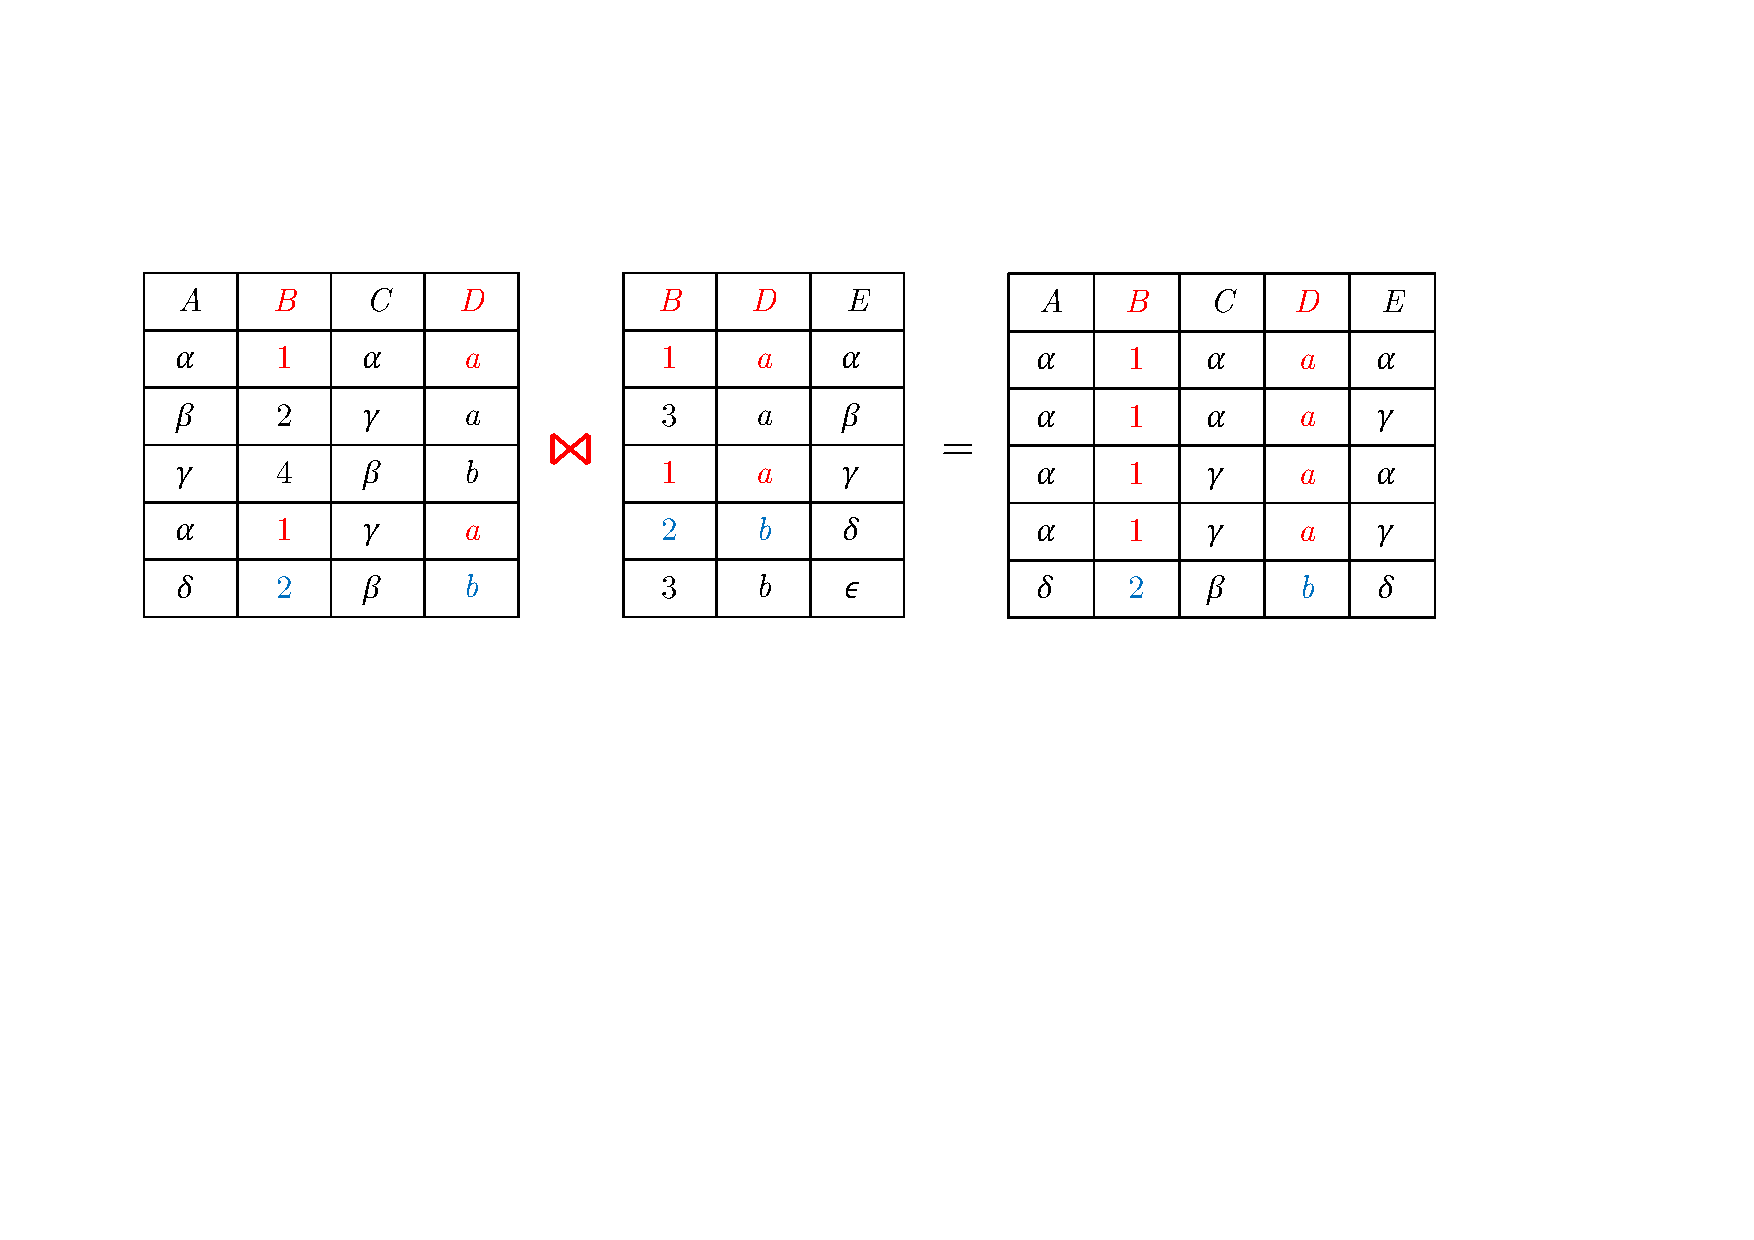
\includegraphics[width=.8\textwidth]{./figure/自然连接.pdf}
    \caption{自然连接例子}
\end{figure}

\begin{example}
求出001号学生所在系的名称:
\begin{align*}
    &\Pi_{\text{dname}}(\sigma_{\text{sno}=001}(S\bowtie \text{Dept})) \\
    &\Pi_{\text{dname}}(\sigma_{\text{sno}=001}(S)\bowtie \text{Dept})
\end{align*}
\end{example}

\begin{example}
关系$R(A,B)$, $S(A,C)$, $R$与$S$中元组个数分别为10, 15, 试填写下表.
\end{example}
\begin{table}[H]
\centering
\begin{tabular}{|c|c|c|c|}
\hline
条件 & 表达式 & 最小元组数 & 最大元组数 \\ \hline
\multirow{2}{*}{无任何条件} & $R \bowtie S$ & 0 & 150 \\ \cline{2-4}
 & $\Pi_A(R) \cup \Pi_A(S)$ & 1 & 25 \\ \hline
\multirow{2}{*}{A是R的主码} & $R \bowtie S$ & 0 & 15 \\ \cline{2-4}
 & $\Pi_A(R) \cup \Pi_A(S)$ & 10 & 25 \\ \hline
\multirow{2}{*}{\begin{tabular}[c]{@{}c@{}}A是R的主码\\ A是S的外码\end{tabular}} & $R \bowtie S$ & 15 & 15 \\ \cline{2-4}
 & $\Pi_A(R) \cup \Pi_A(S)$ & 10 & 10 \\ \hline
\end{tabular}
\caption{不同条件下的表达式及其元组数范围}
\end{table}

自然连接的问题: \textbf{因失配而发生信息丢失}.

\begin{definition}[外连接]
为避免自然连接时因失配而发生的信息丢失, 
可以假定往参与连接的一方表中附加一个取值全为空值的行, 
它和参与连接的另一方表中的任何一个未匹配上的元组都能匹配, 称之为外连接.

外连接 = 自然连接 + 未匹配元组(悬挂元组).

外连接的形式:
\begin{enumerate}
    \item 左外连接 = 自然连接 + 左侧表中未匹配元组. $\leftouterjoin$.
    \item 右外连接 = 自然连接 + 右侧表中未匹配元组. $\rightouterjoin$.
    \item 全外连接 = 左外连接 + 右外连接. $\fullouterjoin$.
\end{enumerate}
\end{definition}

\begin{figure}[H]
    \centering
    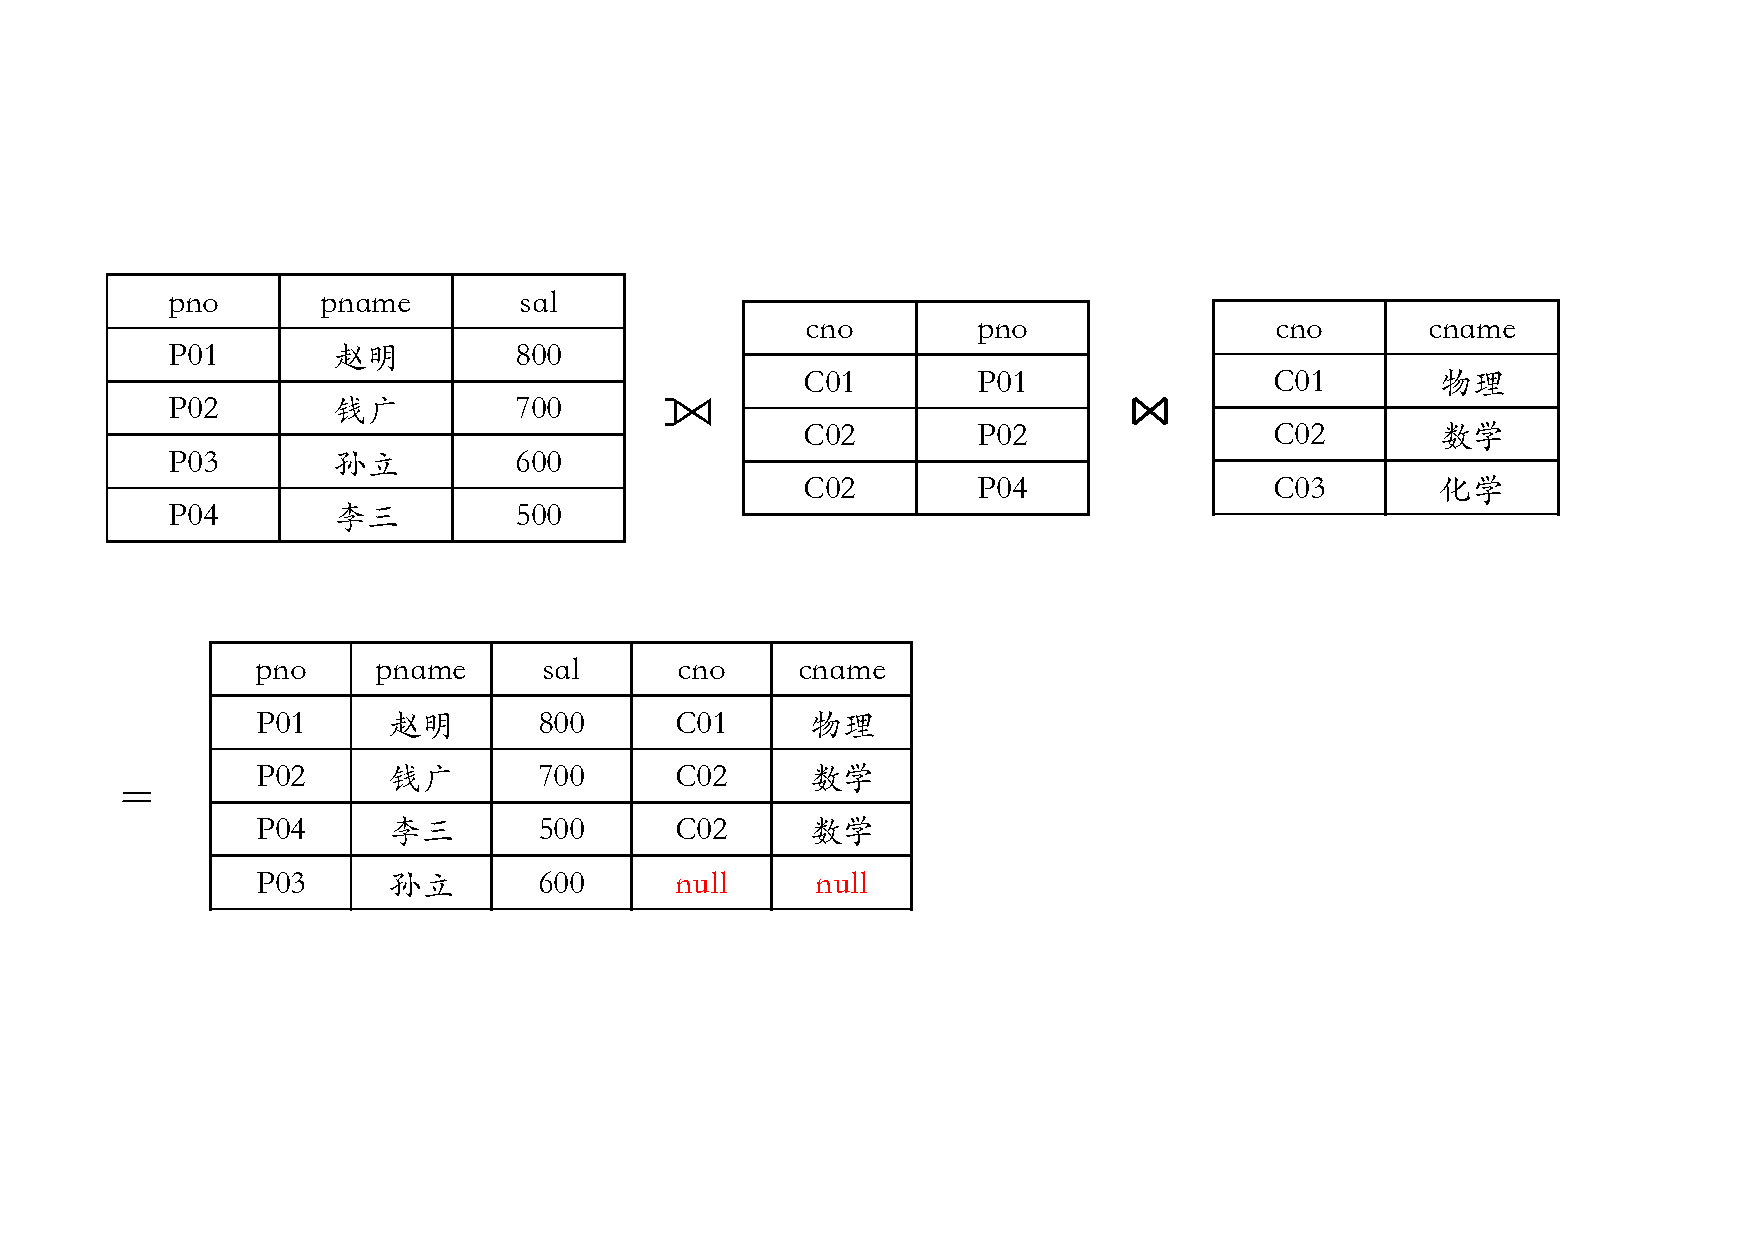
\includegraphics[width=.85\textwidth]{./figure/左外连接.pdf}
    \caption{左外连接示意图}
\end{figure}

外连接结合律不成立的反例:
\begin{figure}[H]
    \centering
    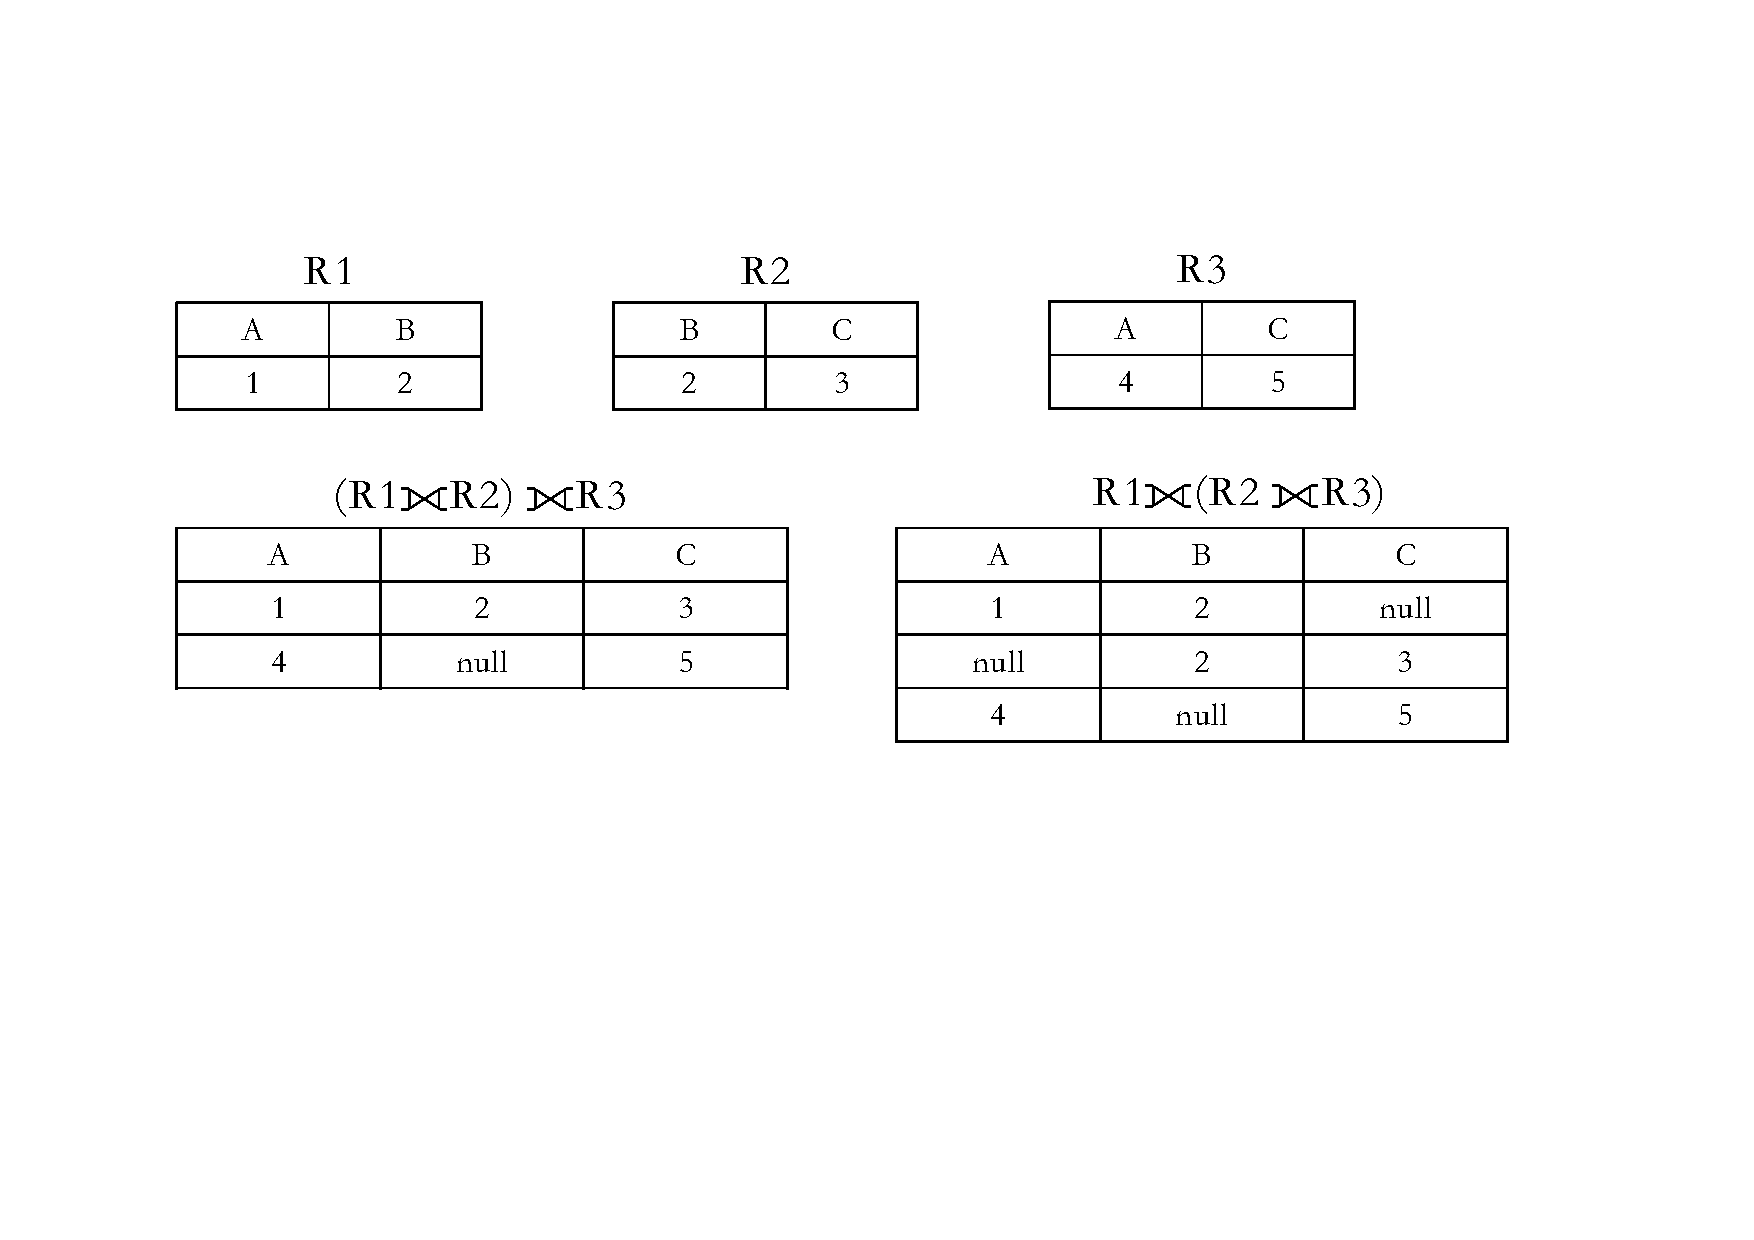
\includegraphics[width=.7\textwidth]{./figure/外连接结合律不成立.pdf}
    \caption{外连接结合律不成立的反例}
\end{figure}

\begin{definition}[半连接]
半连接(Semi-join)是一种用于优化查询的操作, 特别是在分布式数据库系统中. 
它主要用于减少数据传输量, 提高查询效率. 
半连接操作的目标是从两个关系(表)中返回第一个关系中的那些元组(行), 
这些元组与第二个关系中的至少一个元组匹配. $\ltimes$.

简单来说, 半连接操作会从一个表(称为外部表或左表)中选择记录, 
并检查这些记录是否在另一个表(称为内部表或右表)中有对应的记录.
如果有, 则保留该记录; 如果没有, 则丢弃. 
但是, 与普通连接不同的是, 结果集只包含来自外部表的列, 而不包含内部表的任何列.
\end{definition}

半连接可以通过 SQL 查询中的 \verb|EXISTS| 或 \verb|IN| 子查询来实现.

\begin{definition}[反半连接]
在半连接操作中, 我们会从第一个表(外部表或左表)中选出那些在第二个表(内部表或右表)中有匹配记录的行. 
而反半连接则恰恰相反, 它的目的是找出那些在第一个表中存在但在第二个表中没有匹配记录的所有行. $\overline{\ltimes}$.
\end{definition}

在SQL中, 反半连接通常可以通过 \verb|NOT EXISTS| 或者 \verb|LEFT JOIN| 加上 \verb|IS NULL| 的方式来实现.

\begin{figure}[H]
    \centering
    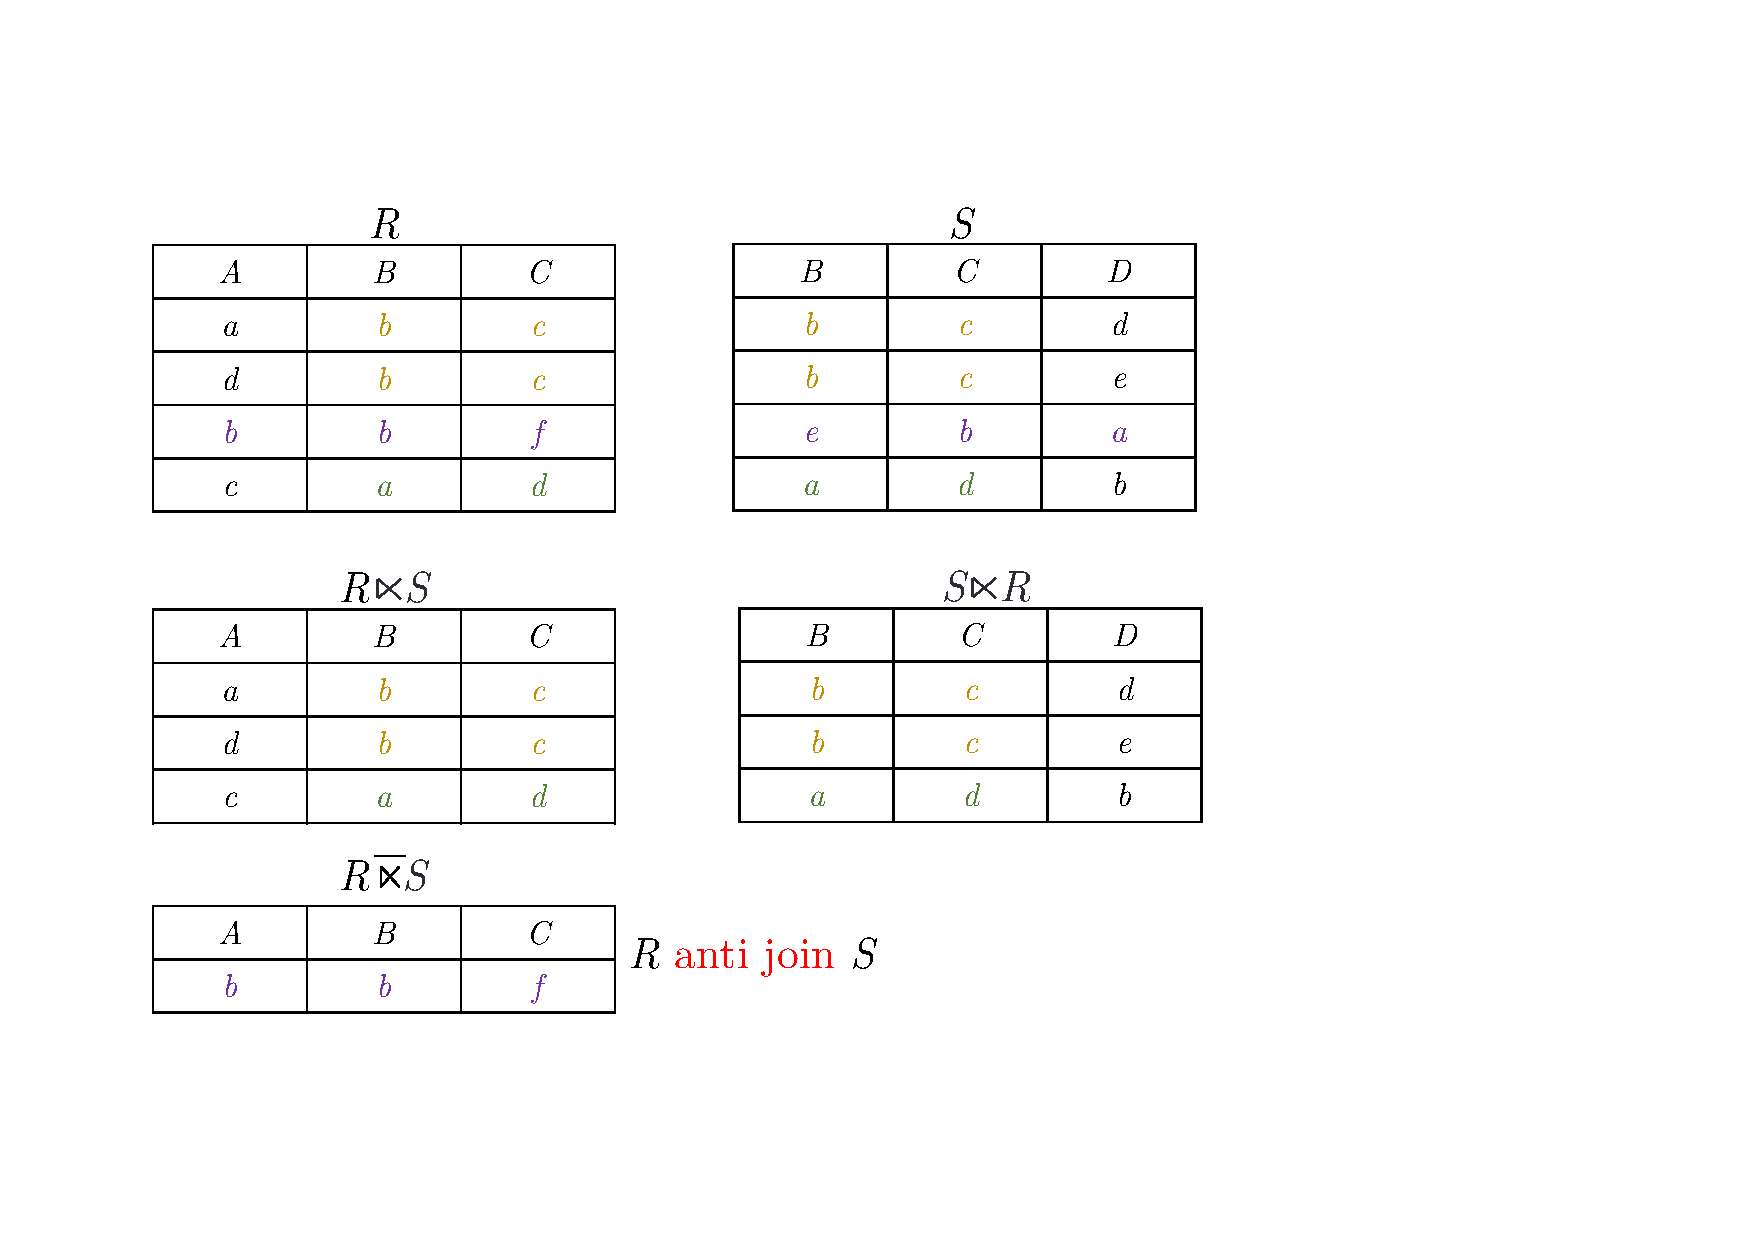
\includegraphics[width=.6\textwidth]{./figure/半连接.pdf}
    \caption{半连接示意图}
\end{figure}

\begin{definition}[外部并]
外部并操作的目标是在保持这种兼容性的同时合并这些关系. 
不过, 与内部并(Inner Union)不同, 外部并也会保留那些在其中一个关系中存在但在另一个关系中不存在的属性值.
\begin{align*}
    R \cup_{\text{outer}} S
\end{align*}
\end{definition}

\begin{figure}[H]
    \centering
    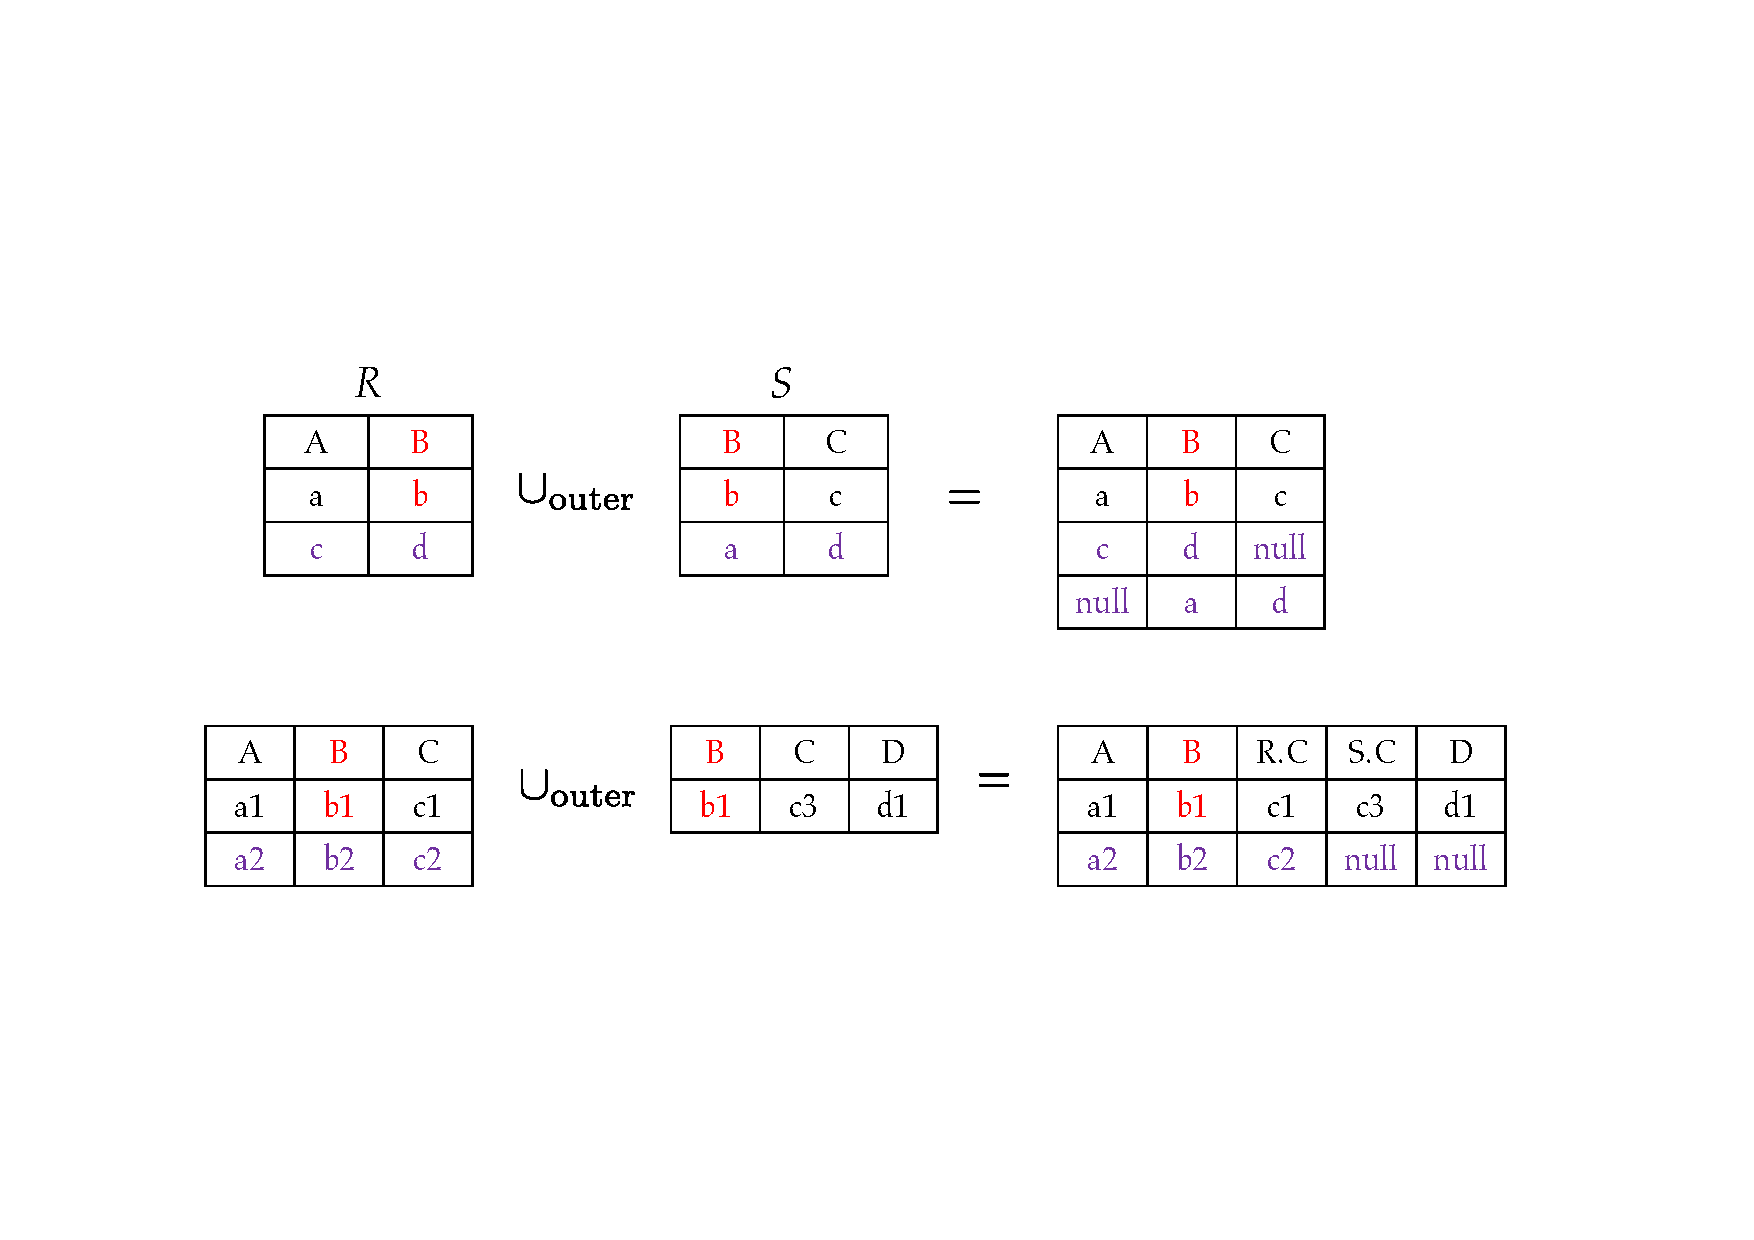
\includegraphics[width=.8\textwidth]{./figure/外部并.pdf}
    \caption{外部并示意图}
\end{figure}

\begin{definition}[象集(Image Set)]
    对于关系$R(X,Z)$, $X,Z$是属性组, $x$是$X$上的取值, 定义$x$在$R$中的\textcolor{red}{象集}为:
\begin{align*}
    Z_x = \{t[Z] | t\in R \land t[X]=x\}
\end{align*}
\end{definition}

\begin{remark}
    象集实际是是: (1)先从$R$中选出在$X$上取值为$x$的元组; (2)只保留$Z$属性.
\end{remark}

\begin{example}
如何求得选修了全部课程的学生?
\end{example}

思路一: 判断每个学生的课程象集是否包含了整个课程集合.
\begin{align*}
    \{u|r\in SC \land u=r[\text{姓名}] \land \text{课程名}_u \supseteq C \}
\end{align*}

思路二: 判断学生与课程集合构成的笛卡尔积是否完全包含在选课集合中.
\begin{align*}
    \{u|r\in SC \land u=r[\text{姓名}] \land \forall c\in C, (u,c)\in SC\}    
\end{align*}

\begin{definition}[除法]
除法通常用来找出在第一个关系中与第二个关系中的所有元素都有匹配的那些元组. 它的定义式为:
\begin{align*}
    &R(X,Y) \div S(Y) = \{x|r\in R\land x=r[X] \land Y_x \supseteq S\}, \\
    &R(X,Y) \div S(Y) = \{u|u\in \Pi_X(R) \land \forall v \in S, \widehat{uv} \in R \}.
\end{align*}
除法的计算表达式为:
\begin{align*}
    R(X,Y) \div S(Y) = \Pi_X(R) - \Pi_X(\Pi_X(R)\times \Pi_Y(S) - R).
\end{align*}
\end{definition}

\begin{example}
对于$SC(sno,cno,grade)$, 求选修了所有课程的学生.
\end{example}

\begin{align*}
    \Pi_{sno,cno}(SC) \div \Pi_{cno}(C)
\end{align*}

现在对于除运算中的被除关系要正确投影:

也就是我们考虑下面的两个式子:
\begin{align*}
    &\Pi_{sno,cno}(SC) \div \Pi_{cno}(C)\\
    &\Pi_{sno}(SC\div \Pi_{cno}(C))
\end{align*}

它们对应着下面的图:
\begin{figure}[H]
    \centering
    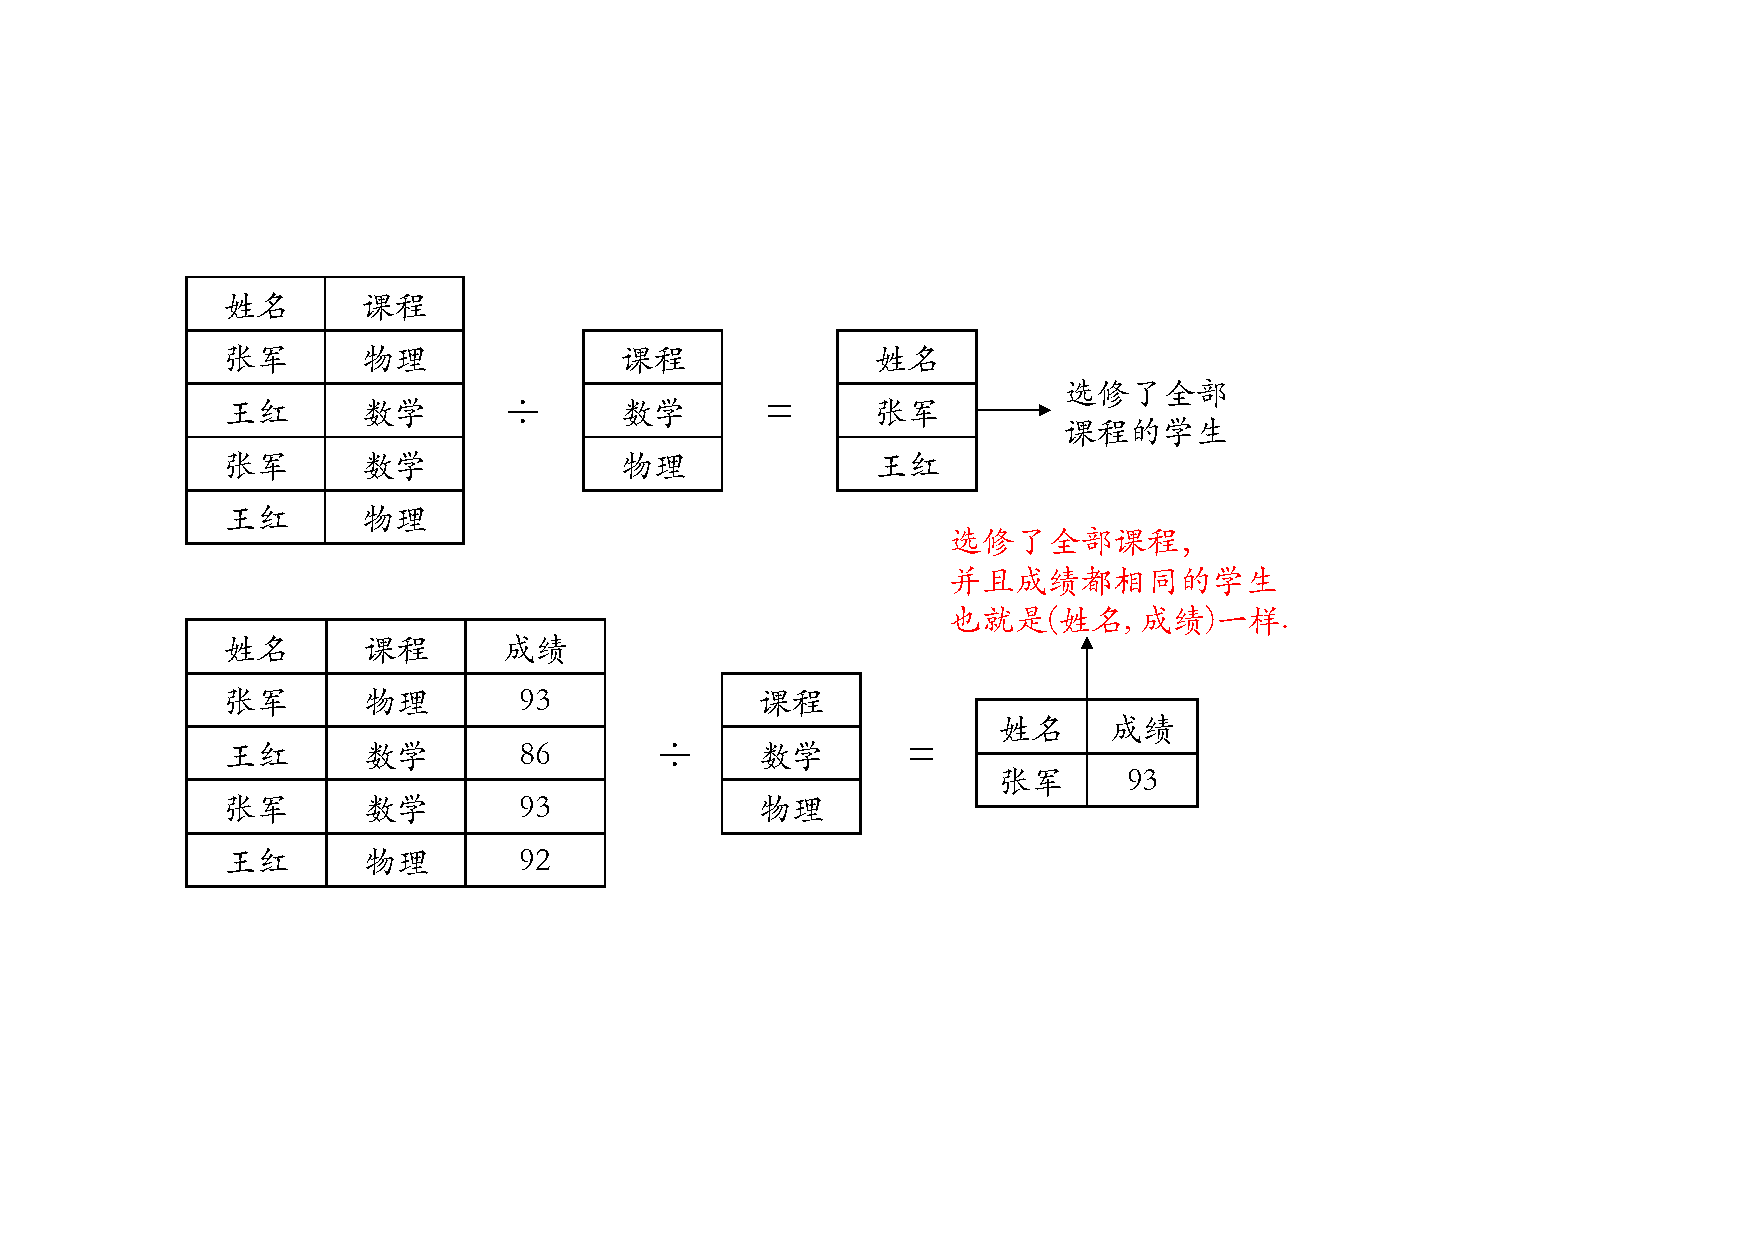
\includegraphics[width=.7\textwidth]{./figure/除法要求.pdf}
    \caption{对于除运算中的被除关系要正确投影}
\end{figure}

\subsection{关系代数更新运算}

\begin{definition}[赋值运算]
为使查询表达简单、清晰, 可以将一个复杂关系代数表达式分成几个部分, 每一部分都赋予一个临时关系变量, 该变量可被看作关系而在后续表达式中使用.
\begin{align*}
    \text{临时关系变量} \leftarrow \text{关系代数表达式}
\end{align*}
\end{definition}

